% dyn_shim — a talk. Beamer, 16:9, dark "oxide" theme.
% Build: latexmk -pdf dyn_shim.tex   (or: pdflatex dyn_shim.tex ×2)
\documentclass[aspectratio=169,11pt,t]{beamer}

\usepackage[T1]{fontenc}
\usepackage[utf8]{inputenc}
\usepackage{FiraSans}
\usepackage[scaled=0.82]{beramono}   % Bera Mono as \ttfamily (no >> ligature)
\renewcommand{\familydefault}{\sfdefault}
\usepackage{listings}
\usepackage{tikz}
\usepackage{ulem}
\usepackage{colortbl}
\usepackage{microtype}
\DisableLigatures[>,<]{encoding = T1, family = tt*}   % kill >> => » in inline mono
\usetikzlibrary{positioning,fit,backgrounds,calc}
\usefonttheme{professionalfonts}

% ─────────────────────────────────────────────────────────── palette
\definecolor{ground}{HTML}{16110D}
\definecolor{panel}{HTML}{1F1813}
\definecolor{term}{HTML}{0F0B08}
\definecolor{line}{HTML}{3A2D22}
\definecolor{linesoft}{HTML}{2B211A}
\definecolor{text}{HTML}{EDE3D4}
\definecolor{muted}{HTML}{A18E7A}
\definecolor{dim}{HTML}{79684F}
\definecolor{oxide}{HTML}{E86A3C}
\definecolor{oxidesoft}{HTML}{D98A66}
\definecolor{steel}{HTML}{8FB6D6}
\definecolor{err}{HTML}{F2555A}
\definecolor{green}{HTML}{A9BE7B}
\definecolor{gold}{HTML}{D6B36A}

% ─────────────────────────────────────────────────────────── theme
\setbeamercolor{normal text}{fg=text,bg=ground}
\setbeamercolor{structure}{fg=oxide}
\setbeamercolor{frametitle}{fg=text,bg=ground}
\setbeamercolor{title}{fg=text}
\setbeamercolor{itemize item}{fg=oxide}
\setbeamercolor{itemize subitem}{fg=dim}
\setbeamerfont{frametitle}{series=\bfseries,size=\Large}
\setbeamerfont{title}{series=\bfseries}
\setbeamertemplate{navigation symbols}{}
\setbeamertemplate{itemize item}{\small\raisebox{0.12ex}{\textbullet}}
\setbeamertemplate{itemize subitem}{\scriptsize\raisebox{0.2ex}{--}}

% eyebrow + rule frametitle
\setbeamertemplate{frametitle}{%
  \vspace*{0.7em}%
  {\usebeamerfont{frametitle}\insertframetitle\par}%
  \vspace*{0.15em}%
  {\color{line}\hrule height 0.6pt}%
  \vspace*{0.2em}%
}

% footline: progress squares + counter
\setbeamertemplate{footline}{%
  \hbox{}\vspace*{0.4em}%
  \hbox to \paperwidth{\hskip1.1em
    \color{dim}\ttfamily\scriptsize
    \insertframenumber\,/\,\inserttotalframenumber
    \hfil
    \color{dim}\scriptsize dyn\_shim
    \hskip1.1em}%
  \vspace*{0.5em}%
}

% ─────────────────────────────────────────────────────────── listings
\lstdefinelanguage{Rust}{
  morekeywords={fn,let,trait,impl,for,where,dyn,mut,use,type,struct,pub,mod,as,match,move,self,Self,ref,const,unsafe},
  morekeywords=[2]{Vec,Box,str,usize,u32,String,Option,Self,Map,Write,Read,Hasher,Hash,Clone,ToOwned,Send,Sync,Parser,Channel,DynChannel,Log,DynLog,Brush,DynBrush,Foo,DynFoo,Widget,DynClone,DynHash,MyTrait,Words,Bytes,Iterator,Item,H,T,F,B},
  morekeywords=[3]{connect,label,deliver,close,parse,build,write_to,thicker,hash,clone,clone_box,draw,new,next,map,sink},
  morekeywords=[4]{dyn_shim,dyn_shim_bind,dyn_shim_foreign,dyn_shim_recognized,reflexive,erase,boxed,panic,stub},
  sensitive=true,
  morecomment=[l]{//},
  morestring=[b]",
}
\lstdefinestyle{rust}{
  language=Rust,
  basicstyle=\ttfamily\small\color{text},
  keywordstyle=\color{oxidesoft},
  keywordstyle=[2]\color{steel},
  keywordstyle=[3]\color{text},
  keywordstyle=[4]\color{oxide}\bfseries,
  commentstyle=\color{dim}\itshape,
  stringstyle=\color{green},
  showstringspaces=false,
  columns=fullflexible,
  keepspaces=true,
  breaklines=false,
  aboveskip=0pt,belowskip=0pt,
  escapeinside={(*}{*)},
}
\lstset{style=rust}

% inline code
\newcommand{\code}[1]{{\ttfamily\small\color{oxidesoft}#1}}
\newcommand{\codet}[1]{{\ttfamily\small\color{text}#1}}

% ─────────────────────────────────────────────────────────── helpers
% eyebrow label above a frame's body
\newcommand{\eyebrow}[2][steel]{{\ttfamily\scriptsize\bfseries\color{#1}\MakeUppercase{#2}}\par\vspace{0.4em}}
% panel box for code
\newcommand{\panelbox}[2][panel]{%
  \begin{tikzpicture}
    \node[fill=#1,draw=line,line width=0.6pt,rounded corners=3pt,
          inner xsep=10pt,inner ysep=8pt,align=left] {#2};
  \end{tikzpicture}}
% a header for a code panel
\newcommand{\panelhd}[1]{{\ttfamily\scriptsize\color{dim}\MakeUppercase{#1}}\\[3pt]}

% lede paragraph
\newcommand{\lede}[1]{{\color{muted}\fontsize{13}{18.5}\selectfont #1\par}}
\newcommand{\ledesm}[1]{{\color{muted}\fontsize{11.3}{16}\selectfont #1\par}}
% note (mono, dim)
\newcommand{\dnote}[1]{{\ttfamily\scriptsize\color{dim}#1\par}}
% oxide emphasis
\newcommand{\ox}[1]{{\color{oxide}#1}}
\newcommand{\tx}[1]{{\color{text}\bfseries#1}}

% ladder row: two columns inside a bordered stack
\newcommand{\ladderrow}[3][panel]{%
  \begin{tikzpicture}
  \node[fill=#1,text width=\dimexpr\linewidth-20pt\relax,inner xsep=10pt,inner ysep=7pt] (r){%
    \begin{minipage}[t]{0.44\linewidth}\small\strut\raggedright #2\end{minipage}%
    \hfill
    \begin{minipage}[t]{0.53\linewidth}\small\strut\raggedright\color{muted} #3\end{minipage}%
  };
  \end{tikzpicture}\vspace{-2pt}}

\begin{document}
\setlength{\parindent}{0pt}

% ═══════════════════════════════════════════════════════ 1 · title
{
\setbeamertemplate{footline}{}
\begin{frame}[plain,c]
\vfill
\eyebrow[dim]{A Rust talk · \,15 minutes}
\vspace{1.2em}

{\ttfamily\LARGE\bfseries\color{text}Vec<Box<{\color{err}\uline{dyn Parser}}>>}\\[0.7em]
{\fontsize{40}{44}\selectfont\bfseries\color{text}The compiler says \ox{no.}}\\[0.9em]
\lede{dyn-compatibility --- what the language already gives you,\\ and how to cheat past the rest.}
\vfill
\dnote{\color{muted}nixpulvis \quad·\quad a talk that ends in a crate}
\end{frame}
}

% ═══════════════════════════════════════════════════════ 2 · the code you wanted
\begin{frame}[fragile]{The code you wanted to write}
\eyebrow{The problem}
\begin{columns}[T]
\begin{column}{0.5\textwidth}
\begin{lstlisting}
trait Parser {
    fn parse(&self, input: &str) -> usize;
    fn build() -> Self;
}

let parsers: Vec<Box<dyn Parser>> = vec![
    Box::new(Words::build()),
    Box::new(Bytes::build()),
];
\end{lstlisting}
\end{column}
\begin{column}{0.5\textwidth}
{\ttfamily\footnotesize
{\color{err}\bfseries error[E0038]}{\color{text}: the trait `Parser'}\\
{\color{text}is not dyn compatible}\\[3pt]
{\color{steel}7 |}\ \ let parsers: Vec<Box<dyn Parser>>\\
{\color{steel}\ \ |}\ \ \ \ \ \ \ \ \ \ \ \ \ \ \ \ \ \ \ \ \ \ {\color{err}\char`\^\char`\^\char`\^\char`\^\char`\^\char`\^ not dyn}\\
{\color{steel}\ \ |}\ \ \ \ \ \ \ \ \ \ \ \ \ \ \ \ \ \ \ \ \ \ \ \ {\color{err}compatible}\\[3pt]
{\color{steel}\ \ = note:} for a trait to be dyn\\
\ \ \ \ compatible it needs to allow\\
\ \ \ \ building a vtable\\[3pt]
{\color{steel}3 |}\ \ \ \ fn build() -> Self;\\
{\color{steel}\ \ |}\ \ \ \ \ \ \ {\color{err}\char`\^\char`\^\char`\^\char`\^\char`\^} ...because associated\\
\ \ \ \ function `build' has no `self'\\
\ \ \ \ parameter\\
}
\end{column}
\end{columns}
\vspace{0.8em}
\dnote{real output --- rustc 1.88, verbatim (lightly wrapped)}
\end{frame}

% ═══════════════════════════════════════════════════════ 3 · vtable
\begin{frame}{There is no slot for \code{build}}
\eyebrow{The problem}
\vspace{0.3em}
\begin{center}
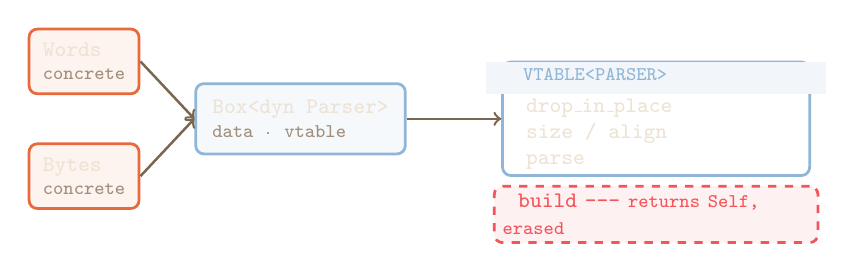
\begin{tikzpicture}[font=\ttfamily\footnotesize,node distance=6mm]
  \node[draw=oxide,line width=1pt,rounded corners=3pt,fill=oxide!8,text=text,inner sep=5pt,align=left] (w) {\textbf{Words}\\[-1pt]{\color{muted}\scriptsize concrete}};
  \node[draw=oxide,line width=1pt,rounded corners=3pt,fill=oxide!8,text=text,inner sep=5pt,align=left,below=of w] (b) {\textbf{Bytes}\\[-1pt]{\color{muted}\scriptsize concrete}};
  \node[draw=steel,line width=1pt,rounded corners=3pt,fill=steel!8,text=text,inner sep=6pt,align=left,right=14mm of $(w)!0.5!(b)$] (fat) {Box<dyn Parser>\\[-1pt]{\color{muted}\scriptsize data · vtable}};
  \node[draw=steel,line width=1pt,rounded corners=3pt,inner sep=0pt,right=12mm of fat,text=text] (vt) {%
    \begin{tabular}{@{}p{3.9cm}@{}}
      \rowcolor{steel!12}\multicolumn{1}{@{}l@{}}{\scriptsize\color{steel}\ \ VTABLE<PARSER>}\\[2pt]
      \ \ drop\_in\_place\\
      \ \ size / align\\
      \ \ parse\\[1pt]
    \end{tabular}};
  \node[draw=err,line width=1pt,dashed,rounded corners=3pt,fill=err!8,text=err,inner sep=3pt,below=1mm of vt.south,anchor=north,text width=3.9cm] (dead) {\ \ build --- {\scriptsize returns Self, erased}};
  \draw[->,dim,line width=0.9pt] (w.east) -- (fat.west);
  \draw[->,dim,line width=0.9pt] (b.east) -- (fat.west);
  \draw[->,dim,line width=0.9pt] (fat.east) -- (vt.west);
\end{tikzpicture}
\end{center}
\vspace{0.4em}
\lede{A vtable is a table of function pointers over an \tx{erased} type. \code{build} returns \code{Self} --- the one thing erasure just deleted.}
\end{frame}

% ═══════════════════════════════════════════════════════ 4 · everything that breaks dyn
\begin{frame}[fragile]{Everything that breaks \code{dyn}}
\eyebrow{The problem}
\ladderrow{\lstinline|fn build() -> Self;|}{returns the erased type}
\ladderrow[linesoft]{\lstinline|fn crunch(self) -> u32;|}{consumes it by value}
\ladderrow{\lstinline|fn write_to(&self, w: &mut impl Write);|}{a different function per \code{W} --- the vtable needs exactly one}
\ladderrow[linesoft]{\lstinline|fn map<F>(self, f: F) -> Map<Self, F>;|}{generic: monomorphized, unbounded set}
\ladderrow{\lstinline|trait Brush: Clone|}{supertrait \code{Clone} requires \code{Sized} --- no method to blame}
\vspace{0.6em}
\dnote{every one of these comes back in the next ten minutes}
\end{frame}

% ═══════════════════════════════════════════════════════ 5 · escape hatch in the error
\begin{frame}[fragile]{The escape hatch ships in the error message}
\eyebrow{What the language gives you}
\vspace{0.2em}
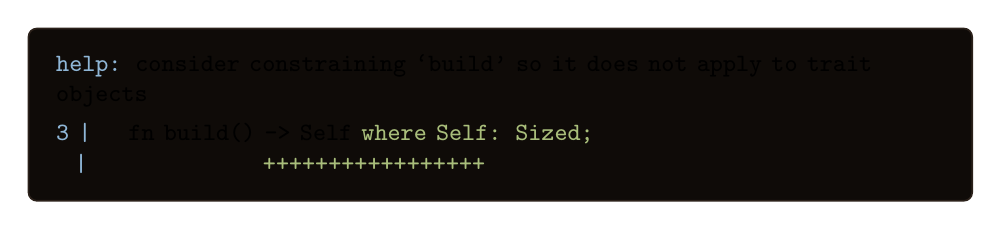
\begin{tikzpicture}
\node[fill=term,draw=linesoft,line width=0.6pt,rounded corners=3pt,inner sep=10pt,text width=\dimexpr\linewidth-24pt\relax]{%
{\ttfamily\small
{\color{steel}help:} consider constraining `build' so it does not apply to trait objects\\[3pt]
{\color{steel}3 |}\ \ \ \ fn build() -> Self {\color{green}\bfseries where Self: Sized;}\\
{\color{steel}\ \ |}\ \ \ \ \ \ \ \ \ \ \ \ \ \ \ \ \ \ \ {\color{green}\bfseries +++++++++++++++++}\\
}};
\end{tikzpicture}
\vspace{0.9em}
\lede{\code{where Self: Sized} on a \tx{method} removes that method from the vtable --- not the trait from \code{dyn}. The trait stays dyn-compatible; the method is only callable on concrete types.}
\vspace{0.4em}
\dnote{common misreading: people assume one bad method poisons the whole trait. It doesn't.}
\end{frame}

% ═══════════════════════════════════════════════════════ 6 · Iterator
\begin{frame}[fragile]{You already rely on this every day}
\eyebrow{What the language gives you}
\begin{columns}[T]
\begin{column}{0.52\textwidth}
\panelhd{std::iter::Iterator}
\begin{lstlisting}
trait Iterator {
    type Item;
    fn next(&mut self)
        -> Option<Self::Item>;

    fn map<B, F>(self, f: F)
        -> Map<Self, F>
    where Self: Sized { (* ... *) }

    // ~70 more adapters, each:
    where Self: Sized
\end{lstlisting}
\end{column}
\begin{column}{0.46\textwidth}
\panelhd{the compiler writes this for free}
\begin{lstlisting}
impl Iterator
  for dyn Iterator<Item=T> { (* ... *) }
\end{lstlisting}
\vspace{1em}
\ledesm{The standard library's biggest trait is dyn-compatible because of this one clause --- and \code{dyn Iterator} satisfies \code{Iterator} automatically, gated methods simply absent.}
\end{column}
\end{columns}
\end{frame}

% ═══════════════════════════════════════════════════════ 7 · punchline
{
\setbeamercolor{background canvas}{bg=ground}
\begin{frame}[plain,c]
\vfill
\begin{center}
\eyebrow[oxide]{Takeaway \textnumero1}
\vspace{0.6em}

{\fontsize{27}{35}\selectfont\bfseries\color{text}If you own the trait,\\ and its objects can live\\ without those methods ---\\[0.35em] \ox{you don't need a crate.}}
\vspace{1.3em}

\lede{\code{where Self: Sized}, done. The rest of this talk\\ is about when that isn't true.}
\end{center}
\vfill
\end{frame}
}

% ═══════════════════════════════════════════════════════ 8 · where it runs out
\begin{frame}{Four walls you eventually hit}
\eyebrow{Where it runs out}
\vspace{0.2em}
\begin{columns}[T]
\begin{column}{0.49\textwidth}
\panelbox{\begin{minipage}{0.9\linewidth}
{\ttfamily\scriptsize\color{oxide}01}\\[2pt]
{\bfseries\color{text}The method is dead, not dispatched}\\[3pt]
{\color{muted}\footnotesize A \code{Self: Sized} method can never be called through the object. Fine for \code{Iterator::map} --- not for a method your callers actually need on erased values.}
\end{minipage}}\\[6pt]
\panelbox{\begin{minipage}{0.9\linewidth}
{\ttfamily\scriptsize\color{oxide}03}\\[2pt]
{\bfseries\color{text}The problem is a supertrait}\\[3pt]
{\color{muted}\footnotesize \code{trait Brush: Clone} --- there is no method to gate. The incompatibility lives on the trait itself.}
\end{minipage}}
\end{column}
\begin{column}{0.49\textwidth}
\panelbox{\begin{minipage}{0.9\linewidth}
{\ttfamily\scriptsize\color{oxide}02}\\[2pt]
{\bfseries\color{text}You don't own the trait}\\[3pt]
{\color{muted}\footnotesize \code{std::hash::Hash}, something from a dependency --- you can't add a where-clause to code you can't edit.}
\end{minipage}}\\[6pt]
\panelbox{\begin{minipage}{0.9\linewidth}
{\ttfamily\scriptsize\color{oxide}04}\\[2pt]
{\bfseries\color{text}\codet{Box<dyn Foo>} is still not a \codet{Foo}}\\[3pt]
{\color{muted}\footnotesize \code{fn eat(x: impl Foo)} rejects your box. Hand-write the impl and the trap springs: the box \tx{is} \code{Sized}, so every gated method is required again.}
\end{minipage}}
\end{column}
\end{columns}
\end{frame}

% ═══════════════════════════════════════════════════════ 9 · enter dyn_shim
\begin{frame}[fragile]{Generate the trait you'd have written by hand}
\eyebrow[oxide]{The crate · dyn\_shim}
\begin{columns}[T]
\begin{column}{0.48\textwidth}
\panelhd{you write}
\begin{lstlisting}
#[dyn_shim(DynChannel)]
trait Channel {
    fn connect() -> Self;
    fn label(&self) -> String;
    fn deliver(&mut self, msg: &str);
    fn close(self) -> u32;
}
\end{lstlisting}
\end{column}
\begin{column}{0.52\textwidth}
\panelhd{the macro generates (simplified)}
\begin{lstlisting}
trait DynChannel {
    fn label(&self) -> String;
    fn deliver(&mut self, msg: &str);
    fn close(self: Box<Self>) -> u32;
    // connect: skipped
}
impl<T: Channel> DynChannel for T { (* /* fwd */ *) }
\end{lstlisting}
\end{column}
\end{columns}
\vspace{0.6em}
\lede{A dyn-compatible twin plus a blanket impl: \tx{every \code{Channel} is already a \code{DynChannel}} --- so \code{Vec<Box<dyn DynChannel>>} holds a mixed set of implementors.}
\end{frame}

% ═══════════════════════════════════════════════════════ 10 · ladder
\begin{frame}[fragile]{Per method: forward, rewrite, or opt in}
\eyebrow[oxide]{The crate · method selection}
\ladderrow{\lstinline|&self  /  &mut self  /  self: Box<Self>|}{forwarded through the vtable unchanged}
\ladderrow[linesoft]{\lstinline|fn f(self)|}{rewritten to \code{self: Box<Self>} --- automatic}
\ladderrow{\lstinline|where Self: Sized|}{already off the vtable --- skipped; \tx{your gate is respected}}
\ladderrow[gold!14!panel]{\lstinline|fn f(&self, w: &mut impl Write)|}{{\color{oxidesoft}\bfseries \#[dyn\_shim(erase)]} --- lower the generic to a trait object}
\ladderrow[gold!14!panel]{\lstinline|fn f(self) -> Self|}{{\color{oxidesoft}\bfseries \#[dyn\_shim(boxed)]} --- return \code{Box<dyn Shim>} instead}
\ladderrow{\lstinline|/* anything else */|}{\code{stub = ...} / \code{panic} / skipped}
\end{frame}

% ═══════════════════════════════════════════════════════ 11 · erase
\begin{frame}[fragile]{Lower the generic to a trait object}
\eyebrow[oxide]{Remediation · erase}
\lstset{basicstyle=\ttfamily\footnotesize\color{text}}
\begin{columns}[T]
\begin{column}{0.5\textwidth}
\begin{lstlisting}
#[dyn_shim(DynLog)]
trait Log {
    #[dyn_shim(erase)]
    fn write_to(&self, out: &mut impl Write);
}

// on the shim:
fn write_to(&self, out: &mut dyn Write);
\end{lstlisting}
\end{column}
\begin{column}{0.5\textwidth}
\ledesm{Sound exactly when the bound gives you \code{impl Write for \&mut dyn Write} --- and std does, for \tx{Hasher, Write, Read}, and friends.}
\vspace{0.7em}
\ledesm{A bound without it \tx{fails at compile time}, at the forwarding call. Impossible erasures are rejected too:}
\vspace{0.4em}
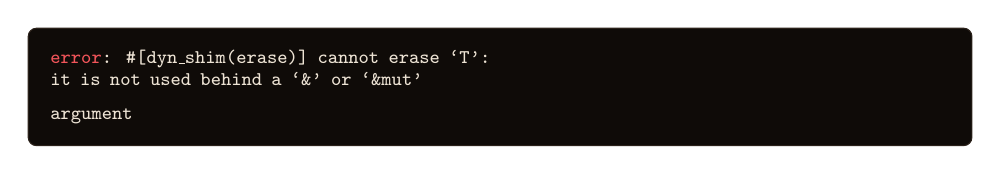
\begin{tikzpicture}
\node[fill=term,draw=linesoft,rounded corners=3pt,inner sep=8pt,text width=\dimexpr\linewidth-20pt\relax]{%
{\ttfamily\scriptsize {\color{err}\bfseries error}{\color{text}: \#[dyn\_shim(erase)] cannot erase `T':\\ it is not used behind a `\&' or `\&mut'\\ argument}}};
\end{tikzpicture}
\end{column}
\end{columns}
\end{frame}

% ═══════════════════════════════════════════════════════ 12 · boxed
\begin{frame}[fragile]{Builders keep building after erasure}
\eyebrow[oxide]{Remediation · boxed}
\begin{columns}[T]
\begin{column}{0.5\textwidth}
\begin{lstlisting}
#[dyn_shim(DynBrush, reflexive = boxed)]
trait Brush {
    #[dyn_shim(boxed)]
    fn thicker(self) -> Self;
}

// on the shim:
fn thicker(self: Box<Self>)
    -> Box<dyn DynBrush>;
\end{lstlisting}
\end{column}
\begin{column}{0.5\textwidth}
\ledesm{The concrete result is boxed and unsized back to the shim object, so a consuming, chaining \code{-> Self} builder still chains on erased values ---}
\vspace{0.5em}
\begin{lstlisting}
let b: Box<dyn DynBrush>
    = b.thicker().thicker();
\end{lstlisting}
\vspace{0.5em}
\ledesm{--- where \code{Self: Sized} would have simply deleted it from the object.}
\end{column}
\end{columns}
\end{frame}

% ═══════════════════════════════════════════════════════ 13 · Clone & Hash are instances
\begin{frame}[fragile]{Clone and Hash aren't features --- they're instances}
\eyebrow[oxide]{The good part}
\lstset{basicstyle=\ttfamily\footnotesize\color{text}}
\vspace{0.2em}
\begin{columns}[c]
\begin{column}{0.44\textwidth}
\begin{lstlisting}
// std::hash::Hash - generic hasher
fn hash<H: Hasher>(&self, s: &mut H);
\end{lstlisting}
\end{column}
\begin{column}{0.1\textwidth}
\begin{center}{\ttfamily\scriptsize\bfseries\colorbox{steel}{\color{ground}\,ERASE\,}}\end{center}
\end{column}
\begin{column}{0.44\textwidth}
\begin{lstlisting}
// the DynHash carrier
fn hash(&self, s: &mut dyn Hasher);
\end{lstlisting}
\end{column}
\end{columns}
\vspace{0.6em}
\begin{columns}[c]
\begin{column}{0.44\textwidth}
\begin{lstlisting}
// std::clone::Clone - returns Self
fn clone(&self) -> Self;
\end{lstlisting}
\end{column}
\begin{column}{0.1\textwidth}
\begin{center}{\ttfamily\scriptsize\bfseries\colorbox{oxide}{\color{ground}\,BOXED\,}}\end{center}
\end{column}
\begin{column}{0.44\textwidth}
\begin{lstlisting}
// the DynClone carrier
fn clone_box(&self) -> Box<dyn DynClone>;
\end{lstlisting}
\end{column}
\end{columns}
\vspace{0.9em}
\lede{The shipped \code{DynClone} / \code{DynHash} carriers are generated by running synthetic signatures through the \tx{same two transforms} user methods get. Two ecosystem crates, as one-liners of the general machinery.}
\end{frame}

% ═══════════════════════════════════════════════════════ 14 · drop-in
\begin{frame}[fragile]{Drop-in: retire \code{dyn-clone} and \code{dyn-hash}}
\eyebrow[oxide]{In practice}
\lstset{basicstyle=\ttfamily\footnotesize\color{text}}
\begin{columns}[T]
\begin{column}{0.5\textwidth}
\panelhd{before --- two deps, two macro calls}
\begin{lstlisting}
(*{\color{dim}\itshape\# Cargo.toml}*)
dyn-clone = "1"
dyn-hash  = "0.2"

use dyn_clone::{clone_trait_object, DynClone};
use dyn_hash::{hash_trait_object, DynHash};

trait MyTrait: DynClone + DynHash { }

clone_trait_object!(MyTrait);
hash_trait_object!(MyTrait);
\end{lstlisting}
\end{column}
\begin{column}{0.5\textwidth}
\panelhd{after --- one dep, one attribute}
\begin{lstlisting}
(*{\color{dim}\itshape\# Cargo.toml}*)
dyn_shim = { version = "0.2",
  features = ["dyn_clone", "dyn_hash"] }

use dyn_shim::{dyn_shim_bind,
    DynClone, DynHash};

#[dyn_shim_bind(DynClone + DynHash)]
trait MyTrait: DynClone + DynHash { }
\end{lstlisting}
\end{column}
\end{columns}
\vspace{0.3em}
\lede{Supertraits stay put; the macro invocations become the attribute --- same behavior, \code{Send}/\code{Sync} variants included.}
\end{frame}

% ═══════════════════════════════════════════════════════ 15 · bind generally
\begin{frame}[fragile]{Carriers mount capabilities onto objects}
\eyebrow[oxide]{dyn\_shim\_bind}
\begin{columns}[T]
\begin{column}{0.5\textwidth}
\begin{lstlisting}
// Foo is NOT dyn-compatible.
// Widget can't have it as a supertrait...

#[dyn_shim_bind(DynFoo)]
trait Widget: DynFoo {
    fn draw(&self);
}

// ...but now dyn Widget satisfies Foo,
// forwarded through the inherited shim.
\end{lstlisting}
\end{column}
\begin{column}{0.5\textwidth}
\ledesm{\code{DynClone} and \code{DynHash} aren't special: \tx{any shim is a carrier}. Inherit it as a supertrait, bind the source trait back onto your objects --- even from another crate.}
\vspace{0.8em}
\ledesm{Contract choice, made visible: a carrier \tx{supertrait} means every implementor must qualify; a recognized bound on a shim merely \tx{filters} which implementors become erasable.}
\end{column}
\end{columns}
\end{frame}

% ═══════════════════════════════════════════════════════ 16 · reflexive
\begin{frame}{Closing the loop back to the source trait}
\eyebrow[oxide]{Reflexive impls}
\lede{The language gives \code{dyn DynFoo: DynFoo} for free --- but nothing ever makes \code{dyn DynFoo: Foo}. Two traits, one gap.}
\vspace{0.6em}
\begin{columns}[T]
\begin{column}{0.49\textwidth}
\panelbox{\begin{minipage}{0.9\linewidth}
{\ttfamily\scriptsize\color{oxide}reflexive = bare}\\[2pt]
{\bfseries\color{text}\codet{impl Foo for dyn DynFoo}}\\[3pt]
{\color{muted}\small Restores the impl the compiler \emph{would have written}, had \code{Foo} been dyn-compatible. Gated methods left off the unsized surface: a compile error, not a runtime panic.}
\end{minipage}}
\end{column}
\begin{column}{0.49\textwidth}
\panelbox[gold!12!panel]{\begin{minipage}{0.9\linewidth}
{\ttfamily\scriptsize\color{oxide}reflexive = boxed}\\[2pt]
{\bfseries\color{text}\codet{impl Foo for Box<dyn DynFoo>}}\\[3pt]
{\color{muted}\small The real feature. \code{Self} is sized, so by-value \code{self} and boxed builders genuinely work --- and the remediation ladder replaces stubs you'd hand-write. Your box now passes into \code{fn eat(x: impl Foo)}.}
\end{minipage}}
\end{column}
\end{columns}
\end{frame}

% ═══════════════════════════════════════════════════════ 17 · two primitives
\begin{frame}[fragile]{Under everything: two primitives}
\eyebrow{Implementation}
\ladderrow{\lstinline|erase_generic(sig)|}{generic param behind \code{\&}/\code{\&mut} $\rightarrow$ trait object --- consumed by \tx{\#[dyn\_shim(erase)]} and the \tx{Hash carrier}}
\ladderrow[linesoft]{\lstinline|build_boxed_method(sig, call)|}{box a \code{Self}-typed result, unsize to \code{Box<dyn Shim + markers>} --- consumed by \tx{\#[dyn\_shim(boxed)]} and the \tx{Clone carrier}}
\vspace{0.7em}
\lede{The user-facing attributes and the shipped carriers are the \tx{same code paths}. The macro is smaller than its feature list --- the features are points in a two-transform space.}
\vspace{0.4em}
\dnote{the Hash carrier is literally a synthetic fn(\&self, \&mut impl Hasher) run through erase\_generic}
\end{frame}

% ═══════════════════════════════════════════════════════ 18 · unsafe
\begin{frame}{The one unsafe block: fat-pointer surgery}
\eyebrow{Implementation}
\vspace{0.3em}
\begin{center}
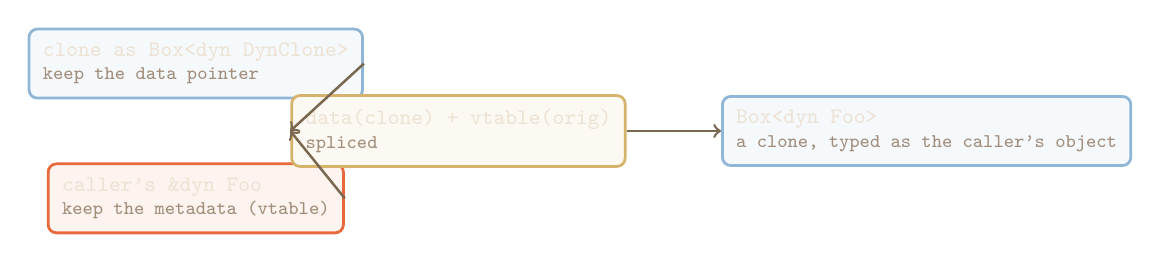
\begin{tikzpicture}[font=\ttfamily\footnotesize,node distance=8mm]
  \node[draw=steel,line width=1pt,rounded corners=3pt,fill=steel!8,text=text,inner sep=5pt,align=left] (c) {clone as Box<dyn DynClone>\\[-1pt]{\color{muted}\scriptsize keep the \textbf{data} pointer}};
  \node[draw=oxide,line width=1pt,rounded corners=3pt,fill=oxide!8,text=text,inner sep=5pt,align=left,below=of c] (o) {caller's \&dyn Foo\\[-1pt]{\color{muted}\scriptsize keep the \textbf{metadata} (vtable)}};
  \node[draw=gold,line width=1pt,rounded corners=3pt,fill=gold!8,text=text,inner sep=5pt,align=left,right=12mm of $(c)!0.5!(o)$] (s) {data(clone) + vtable(orig)\\[-1pt]{\color{muted}\scriptsize spliced}};
  \node[draw=steel,line width=1pt,rounded corners=3pt,fill=steel!8,text=text,inner sep=5pt,align=left,right=12mm of s] (r) {\textbf{Box<dyn Foo>}\\[-1pt]{\color{muted}\scriptsize a clone, typed as the caller's object}};
  \draw[->,dim,line width=0.9pt] (c.east) -- (s.west);
  \draw[->,dim,line width=0.9pt] (o.east) -- (s.west);
  \draw[->,dim,line width=0.9pt] (s.east) -- (r.west);
\end{tikzpicture}
\end{center}
\vspace{0.5em}
\lede{The carrier can only produce \code{Box<dyn DynClone>}; the caller wants \code{Box<dyn Foo>}. Same allocation, same concrete type --- only the metadata differs. So splice the fresh data pointer into the original's metadata, with an \code{assert\_eq!} pinning the layout assumption.}
\vspace{0.3em}
\dnote{src/lib.rs::\_\_clone\_box --- contained, commented, the only unsafe in the crate}
\end{frame}

% ═══════════════════════════════════════════════════════ 19 · errors are the API
\begin{frame}{For a proc macro, the errors \emph{are} the API}
\eyebrow{Implementation}
\vspace{0.2em}
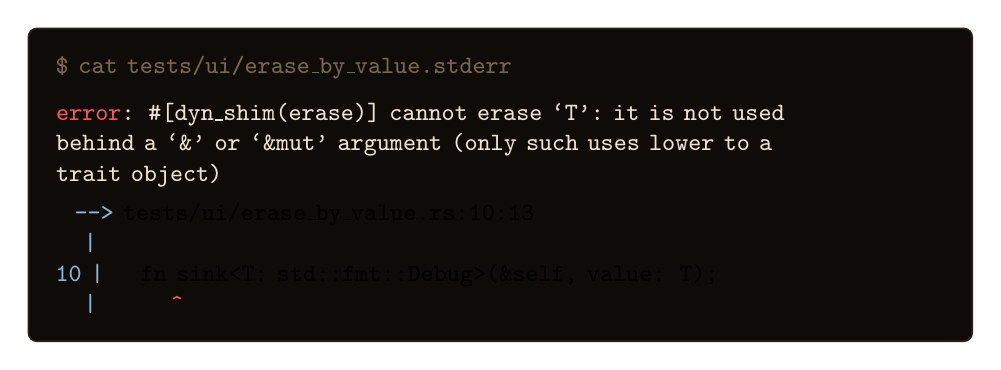
\begin{tikzpicture}
\node[fill=term,draw=linesoft,line width=0.6pt,rounded corners=3pt,inner sep=10pt,text width=\dimexpr\linewidth-24pt\relax]{%
{\ttfamily\small
{\color{dim}\$ cat tests/ui/erase\_by\_value.stderr}\\[6pt]
{\color{err}\bfseries error}{\color{text}: \#[dyn\_shim(erase)] cannot erase `T': it is not used}\\
{\color{text}behind a `\&' or `\&mut' argument (only such uses lower to a}\\
{\color{text}trait object)}\\[3pt]
{\color{steel}\ \ -->} tests/ui/erase\_by\_value.rs:10:13\\
{\color{steel}\ \ \ |}\\
{\color{steel}10 |}\ \ \ \ fn sink<T: std::fmt::Debug>(\&self, value: T);\\
{\color{steel}\ \ \ |}\ \ \ \ \ \ \ \ {\color{err}\char`\^}\\
}};
\end{tikzpicture}
\vspace{0.8em}
\lede{\tx{41 trybuild UI tests} pin the exact wording of every rejection --- each impossible trait, method, and erasure fails with a diagnostic that says \emph{why}, at the right span. Change the message, break the build.}
\end{frame}

% ═══════════════════════════════════════════════════════ 20 · decision ladder
\begin{frame}[fragile]{The decision ladder}
\eyebrow[dim]{Recap}
\ladderrow{\lstinline|where Self: Sized|}{\tx{own the trait, objects can lose the methods} --- the language has you; no dependency}
\ladderrow[linesoft]{\lstinline|#[dyn_shim(DynFoo)]|}{\tx{methods must dispatch}, or you need \code{Box<dyn>: Foo} --- shim + erase / boxed / reflexive}
\ladderrow{\lstinline|#[dyn_shim_foreign(path::Foo)]|}{\tx{the trait isn't yours} --- restate it, the macro forwards and blanket-impls}
\ladderrow[linesoft]{\lstinline|#[dyn_shim_bind(DynClone + ..)]|}{\tx{trait is fine, objects need Clone / Hash / Foo} --- mount capabilities in place}
\vspace{0.4em}
\lede{Rung one is the language; the crate is rungs two through four.}
\end{frame}

% ═══════════════════════════════════════════════════════ 21 · close
{
\setbeamertemplate{footline}{}
\begin{frame}[plain,c]
\vfill
\begin{center}
\eyebrow[dim]{Fin}
\vspace{0.6em}

{\fontsize{40}{46}\selectfont\bfseries\color{text}You might not need \ox{dyn\_shim}.}
\vspace{1em}

{\Large\color{muted}But now you know what it's for.}
\end{center}
\vfill
\dnote{\color{muted}github.com/nixpulvis/dyn\_shim \quad·\quad crates.io/crates/dyn\_shim \quad·\quad questions?}
\end{frame}
}

\end{document}
